Figure \ref{fig:model_composition} gives a summary of the modelling components and their interactions.
\begin{figure}[h]
  \centering
  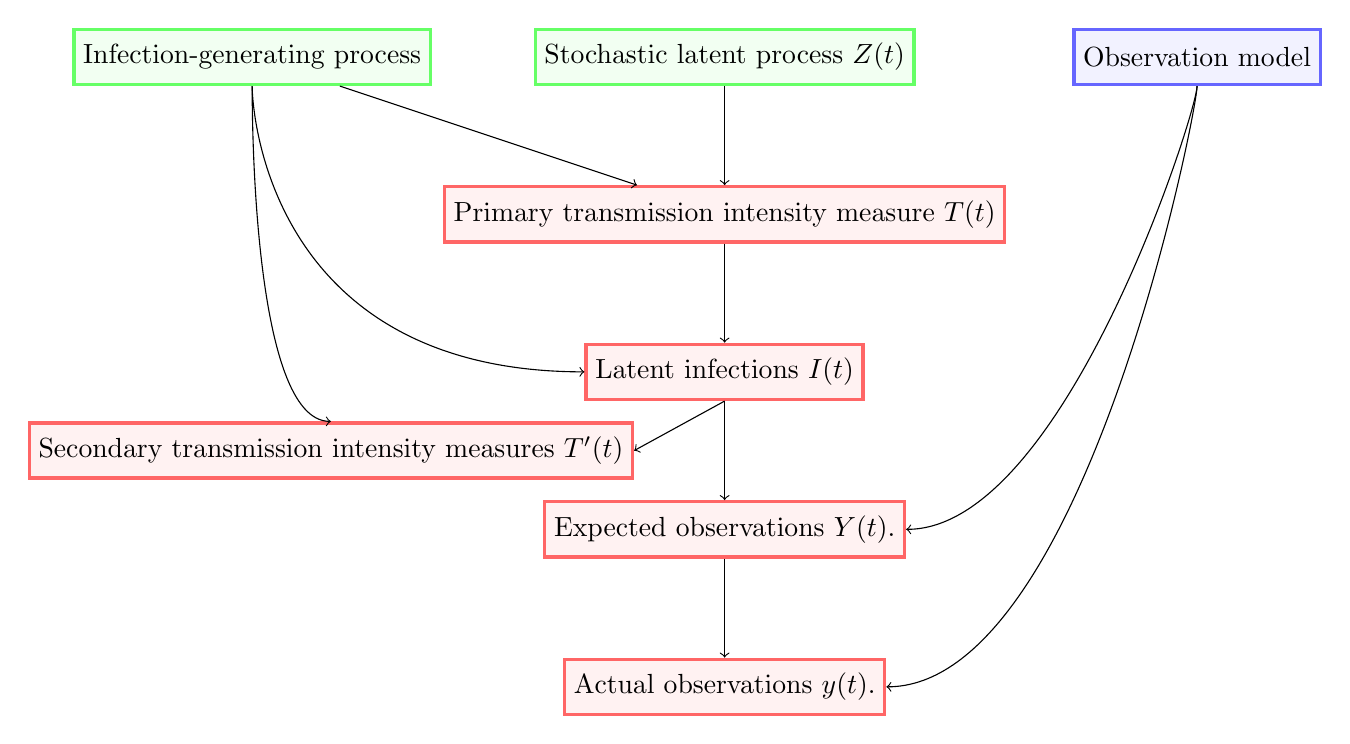
\begin{tikzpicture}[node distance=2cm,
gen_qaunt/.style={draw=red!60, fill=red!5, very thick, minimum size=7mm}, model_spec/.style={draw=green!60, fill=green!5, very thick, minimum size=7mm}, fixed_model_spec/.style={draw=blue!60, fill=blue!5, very thick, minimum size=7mm}]
    % Nodes
    \node (IGP) [draw, model_spec] {Infection-generating process};
    \node (Z) [right of=IGP, xshift=4cm, draw, model_spec] {Stochastic latent process $Z(t)$};
    \node (Obs) [right of=Z, xshift=4cm, draw, fixed_model_spec] {Observation model};
    \node (T) [below of=Z, xshift=0cm, draw, gen_qaunt] {Primary transmission intensity measure $T(t)$};
    \node (I) [below of=T, xshift=0cm, draw, gen_qaunt] {Latent infections $I(t)$};
         \node (T_other) [left of=I, xshift=-3cm, yshift=-1cm,draw, gen_qaunt] {Secondary transmission intensity measures $T'(t)$};
    \node (Y) [below of=I, draw, gen_qaunt] {Expected observations $Y(t)$.};
    \node (yt) [below of=Y, draw, gen_qaunt] {Actual observations $y(t)$.};

    % Arrows
    \draw[->] (IGP) -- node{} (T);
    \draw[->] (Z) -- node{} (T);
    \draw[->] (T) -- node{} (I);
    \draw[->] (IGP) .. controls +(down:7mm) and +(left:4cm) .. (I.west);
    \draw[->] (Obs) .. controls +(down:7mm) and +(right:2cm) .. (Y.east);
    \draw[->] (Obs) .. controls +(down:7mm) and +(right:2.5cm) .. (yt.east);
    % \draw[->] (G.south)  -- node{} (T_other.north);
    % \draw[->] (IGP.south)  -- node{} (T_other.north);
    \draw[->] (IGP) .. controls +(down:7mm) and +(left:1cm) .. (T_other.north);
    \draw[->] (I.south) -- node{} (T_other.east);
    \draw[->] (I) -- node{} (Y);
    \draw[->] (Y) -- node{} (yt);
    
  \end{tikzpicture}
  \caption{Directed graph representing the generative model components. Shown are model choices we experiment over in this study (green rectangles), the observation model (which is fixed in this study; blue rectangle), and generated quantities (red boxes). The generated quantities are split between a primary transmission intensity measure $T(t)$ which composes with the infection-generating process to generate latent infections, and secondary transmission intensity measures.  All transmission intensity measures are targets for surveillance. Each modelled quantity can be constructed conditional on parent quantities on the graph (directed edges).  }
  \label{fig:model_composition}
\end{figure}
